\documentclass[conference]{IEEEtran}

% ------------------------------------------------------------
% Packages
% ------------------------------------------------------------
\usepackage{amsmath,amssymb,amsfonts}
\usepackage{algorithm}
\usepackage{algorithmic}
\usepackage{array}
\usepackage{booktabs}
\usepackage{graphicx}
\usepackage{textcomp}
\usepackage{xcolor}
\usepackage{url}
\usepackage{hyperref}
\usepackage{multirow}
\usepackage{enumitem}
\usepackage{graphicx}
\usepackage{booktabs}

% ------------------------------------------------------------
% Paper information
% IMPORTANT:
% IPDPS 2027 uses double-anonymous review.
% Do not include author names, affiliations, or identifying
% information in the submission version.
% ------------------------------------------------------------

\title{Evaluating LLM Agents for Autonomous Scientific Workflows on HPC Systems}

% Anonymous submission:
% \author{
% \IEEEauthorblockN{Anonymous Authors}
% }

\begin{document}

\maketitle

% ------------------------------------------------------------
% Abstract
% ------------------------------------------------------------


\begin{abstract}
Large language model (LLM) agents hold great promise for advancing scientific discovery by enabling computational tasks to be planned, executed, and iteratively refined based on observed results. However, turning this promise into truly autonomous scientific discovery remains challenging. Scientific discovery is an open-ended process that requires an agent to make a sequence of interdependent decisions, interact with scientific software and data, operate computational resources, respond to failures and unexpected results, and determine what to do next. High-performance computing (HPC) systems further increase this complexity because successful execution requires simultaneously satisfying scientific requirements and system constraints. An agent must therefore reason not only about what computation is scientifically appropriate, but also about whether the selected application, inputs, resources, and execution procedure are mutually compatible with the target HPC environment. Systematically understanding and evaluating these capabilities is an important step toward reliable autonomous scientific discovery.

We present \textit{Trinity}, a multi-agent framework for autonomous scientific discovery that connects LLM-based agents with scientific applications, HPC systems, data-management services, execution interfaces, and system- and application-level observations. Starting from a high-level scientific objective, Trinity enables agents to plan computational workflows, select and prepare scientific applications and inputs, select compatible HPC resources, construct and execute jobs, monitor execution, diagnose failures, analyze results, and determine subsequent scientific actions. This iterative integration of reasoning and computational execution allows Trinity to support scientific workflows that extend beyond one-shot job submission toward autonomous experimentation and discovery. Within this broader framework, we develop a benchmark for evaluating the foundational capability of constructing valid scientific HPC workflows before execution.

The benchmark focuses on four pre-submission capabilities: scientific software selection, input preparation, resource selection, and batch-job creation. We construct diverse instances spanning scientific applications and HPC systems and evaluate agent outputs using domain-aware judging skills that assess constraint satisfaction rather than textual similarity to a single reference solution. This approach accommodates multiple valid solutions while enabling subtask-level failure analysis. The judging skills are iteratively refined through human feedback to identify missing, incorrect, and overly restrictive constraints. Trinity also provides a framework for investigating inference-time capability augmentation using additional context, examples, reusable skills, tools, and external feedback without modifying model parameters.

Our evaluation of four LLMs across 80 benchmark instances shows substantial variation in capability across workflow stages. Resource selection and software selection are generally handled more reliably, while input preparation presents a pronounced challenge across models. The results demonstrate the importance of evaluating scientific HPC agents at the subtask level and highlight the need for domain-specific knowledge and inference-time mechanisms to address capability gaps. Trinity provides a foundation for systematically evaluating and improving LLM agents toward autonomous scientific workflows on large-scale HPC systems.
\end{abstract}

\begin{IEEEkeywords}
HPC, autonomous scientific discovery, scientific workflows,
LLM agents, high-performance computing, agentic systems
\end{IEEEkeywords}

\section{Introduction}\label{sec:introduction}

Large language models (LLMs) are increasingly being developed as agents that can reason about complex tasks, interact with external tools, observe the resulting environment, and iteratively determine subsequent actions. This capability creates new opportunities for automating scientific workflows, where progress from a scientific question to a result often requires a sequence of computational and reasoning steps rather than a single program or answer. An agent may need to identify an appropriate scientific method, prepare inputs, execute computations, inspect results, diagnose failures, and determine what to do next. Recent scientific-agent research has therefore begun to explore the possibility of using LLM-based agents to automate substantial portions of scientific discovery, while also highlighting the need for rigorous evaluation of individual capabilities before making claims about end-to-end scientific automation~\cite{chen2025scienceagentbench}. High-performance computing (HPC) provides an important infrastructure for such workflows, enabling scientific applications to operate at scales that are difficult to achieve on conventional computing systems. At the same time, HPC introduces additional constraints that an autonomous scientific agent must understand before its decisions can be executed successfully.

A central challenge is that scientific HPC workflows require reasoning across two tightly coupled sources of context: the \textit{scientific application context} and the \textit{HPC system context}. The scientific application context includes application semantics, input formats, scientific parameters, execution models, dependencies, and application-specific performance characteristics. The HPC system context includes hardware architecture, installed software, scheduler policies, queue limits, resource configurations, filesystems, and execution procedures. These contexts cannot be treated independently. The scientific application constrains which inputs and execution strategies are meaningful, while the target HPC system constrains which application implementations, resources, and execution procedures are feasible. Consequently, an agent can possess correct knowledge of either domain while still producing an invalid workflow. For example, an agent may select a scientifically appropriate application that is unavailable on the target system, generate a valid application input but request resources incompatible with its parallel execution model, or produce a syntactically valid batch script that does not correctly connect the selected application, inputs, and resources. The resulting problem is therefore not simply HPC resource management or scientific code generation; it is a cross-domain reasoning problem in which a workflow must satisfy coupled scientific and system constraints.

Existing agent systems demonstrate important pieces of this capability, but address different layers of the problem. General agent frameworks provide mechanisms for reasoning, tool use, multi-agent coordination, and reusable skills. Systems connecting LLM agents with scientific computing have demonstrated how agents can invoke scientific applications on HPC resources. For example, Ma et al.~\cite{ma2025langchainparsl} integrate Parsl with LangChain and LangGraph to execute agent-invoked tools concurrently on local and HPC resources, including molecular-dynamics simulations on Polaris. Diamond Agent~\cite{diamondagent2026} further demonstrates agentic orchestration of workloads across heterogeneous HPC resources, using resource discovery, resource specification, data movement, execution, and live system information to support federated HPC execution. These systems demonstrate that agents can interact with and orchestrate computational infrastructure. However, they do not directly address the broader evaluation question of whether an agent can transform a high-level scientific objective into a valid workload by jointly reasoning about the scientific application and the target HPC system. Similarly, HPC operational benchmarks such as AOBench evaluate whether agents can perform operational tasks involving scheduling, telemetry, energy reasoning, policy enforcement, and HPC-native tools~\cite{aobench}, rather than whether an agent can construct a scientifically valid workload for execution on an HPC system.

Evaluating this capability presents several challenges. First, scientific HPC workflow construction may not have a single correct answer. Multiple scientific applications, input configurations, resource allocations, and batch-job scripts can satisfy the same scientific objective. Therefore, textual similarity to a reference solution is insufficient for determining correctness. Instead, evaluation must determine whether a candidate satisfies the scientific and system constraints of the task. Second, the artifacts generated at different stages are coupled. An incorrect software choice can invalidate input preparation, an incorrect input can make an otherwise valid resource configuration unusable, and an inconsistent combination of application, inputs, and resources can result in an invalid batch job. Evaluating only the final artifact can therefore obscure the source of an agent's failure. Third, determining correctness requires domain knowledge. A judge must understand not only generic syntax and execution requirements, but also application-specific semantics and the constraints imposed by the target HPC system. These challenges motivate an evaluation methodology that decomposes scientific HPC workflow construction into meaningful subtasks while retaining the dependencies among their scientific and system constraints.

We present \textit{Trinity}, a multi-agent framework for autonomous scientific discovery and execution across high-performance computing environments. Trinity enables LLM-based agents to transform high-level scientific objectives into executable workflows, interact with scientific applications and HPC infrastructure, observe computational results, and use those observations to determine subsequent actions. The broader goal of Trinity is to support autonomous scientific discovery in which agents can iteratively plan experiments, execute computations, analyze results, diagnose failures, and refine scientific workflows. A complete Trinity workflow can therefore extend beyond job submission to include data and environment preparation, execution and monitoring, failure diagnosis and recovery, result analysis, scientific reasoning, and report generation. In this paper, we focus on a foundational capability required by this broader vision: constructing a valid scientific HPC workload from a high-level scientific objective. We evaluate this capability through four pre-submission stages: scientific software selection, input preparation, resource selection, and batch-job creation. Together, these stages capture the decisions required to translate scientific intent into an executable HPC workload while providing a controlled setting for identifying where and why agents fail.

To enable rigorous evaluation, we develop a benchmark that represents each task through a scientific application and a target HPC system and evaluates the agent's decisions against the coupled constraints of both domains. Each subtask is evaluated independently so that failures can be localized to specific capabilities, while the relationship among subtasks captures the potential for errors to propagate through the workflow. Because multiple valid solutions may exist, Trinity uses domain-aware judging skills to evaluate constraint satisfaction rather than textual similarity to a single reference answer. These judging skills specify the properties and constraints that must be satisfied by a candidate solution and are iteratively refined through human feedback to identify missing, incorrect, or overly restrictive judging rules. The benchmark also provides a basis for studying inference-time capability augmentation: when an agent fails because of missing knowledge, examples, procedural guidance, reusable skills, or other capabilities, additional context and examples can be supplied without modifying the model parameters. This enables the benchmark to evaluate not only the initial capabilities of agents, but also how effectively identified capability gaps can be addressed at inference time.

Our contributions are as follows:
\begin{itemize}
\item \textbf{Trinity framework for autonomous scientific discovery.} We present a multi-agent framework that connects LLM-based reasoning with scientific applications, HPC systems, data-management services, execution infrastructure, monitoring, and scientific feedback to support iterative scientific workflows.

```
\item \textbf{Scientific HPC workflow benchmark.} We develop a benchmark covering four critical pre-submission capabilities---software selection, input preparation, resource selection, and batch-job creation---across diverse scientific applications and HPC systems. The benchmark explicitly captures the coupled constraints between scientific applications and HPC environments.

\item \textbf{Constraint-based and domain-aware evaluation.} We introduce reusable judging skills that evaluate candidate solutions based on scientific and system constraints rather than textual similarity to a single reference answer. Human feedback is used to iteratively refine these judging skills and support the evaluation of heterogeneous valid solutions.

\item \textbf{Subtask analysis and inference-time capability augmentation.} We analyze agent performance at the subtask level to identify capability gaps and investigate whether additional context, examples, reusable skills, tools, and external feedback can improve open-weight agents without modifying their model parameters.
```

\end{itemize}

\section{Background and Related Work}\label{sec:related}

\subsection{AI Agents}

LLM-based agents reason about tasks, invoke external tools, and act on resulting observations, following the interaction pattern established by ReAct~\cite{yao2023react} and extended by multi-agent orchestration frameworks such as AutoGen~\cite{wu2024autogen}. Other work augments agents with externally maintained skills and knowledge without modifying model parameters. For example, Voyager maintains an executable skill library and improves it through environmental feedback~\cite{wang2023voyager}. This separation between model parameters and externally supplied knowledge is particularly relevant to scientific computing, where facility-specific software, system configurations, and application knowledge can change over time. Scientific HPC agents therefore require not only general agentic reasoning and tool use, but also reasoning over application semantics, input requirements, system architecture, software availability, scheduler policies, resource limits, and execution procedures.

\subsection{Scientific and HPC Agents}

Recent work applies LLM agents to scientific and HPC workflows. Ma et al.\ integrate Parsl with LangChain/LangGraph so an LLM agent can invoke scientific tools distributed across HPC resources, demonstrating molecular-dynamics workflows on Polaris~\cite{ma2025langchainparsl}. Diamond Agent instead focuses on workload placement across heterogeneous, independently administered supercomputers using live system and queue information~\cite{diamondagent2026}. Other work studies agents for workflow provenance~\cite{souza2025provenance}, while ECAS separates agent reasoning from execution-side control so that proposed artifacts can be validated before production execution~\cite{sun2026ecas}. These systems primarily focus on executing, orchestrating, placing, or validating workflows, whereas Trinity evaluates whether an agent can \textit{construct} a valid workflow from a high-level objective.

Related work also generates or transforms individual HPC artifacts. ParEval evaluates LLM-generated parallel programs across programming models~\cite{nichols2024pareval}, while HPC-Coder and HPC-Coder-V2 develop models specialized for parallel and scientific computing~\cite{nichols2024hpccoder,chaturvedi2025hpccoderv2}. Sochat and Milroy study translation between Slurm and Flux job specifications~\cite{sochat2026descriptive}. Trinity considers a different artifact-construction problem: selecting an application, preparing its inputs, selecting appropriate resources, and constructing a batch-job specification for a target system. These decisions are coupled because correctness depends simultaneously on the \textit{scientific application context} and the \textit{HPC system context}. An application may be scientifically appropriate but unavailable on the target system, or a system-valid resource configuration may be incompatible with the application's requirements. Trinity therefore treats workflow construction as a \textit{cross-domain constraint-satisfaction problem}.

\subsection{Agent Benchmarks and Evaluation}

General-purpose agent benchmarks establish the importance of evaluating agents through realistic interactions and task outcomes. AgentBench evaluates multi-turn decision-making across interactive environments~\cite{liu2023agentbench}, WebArena evaluates action sequences that change and verify environment state~\cite{zhou2024webarena}, and SWE-bench evaluates repository-level code changes through executable tests~\cite{jimenez2024swebench}. Domain-specific benchmarks extend this methodology to engineering and scientific tasks: MLE-bench evaluates ML engineering~\cite{chan2025mlebench}, MLAgentBench evaluates ML experimentation as a sequence of research actions~\cite{huang2024mlagentbench}, and ScienceAgentBench evaluates scientific discovery through generated programs and expert-informed judgments~\cite{chen2025scienceagentbench}. PaperBench evaluates research-paper reproduction through fine-grained rubric-based subtasks and artifact execution~\cite{starace2025paperbench}.

Several benchmarks further demonstrate the value of decomposing complex agent tasks into intermediate capabilities. AgentBoard evaluates progress against explicit subgoals~\cite{ma2024agentboard}, while CORE-Bench uses multiple levels of computational reproducibility~\cite{siegel2024corebench}. SUPER similarly separates individual research subtasks from end-to-end execution and shows that success on individual components does not necessarily imply successful composition~\cite{bogin2024super}. Trinity applies this stage-decomposed perspective to scientific-HPC workflow construction, using distinct artifacts---application selection, input preparation, resource selection, and batch-job creation---rather than trajectory checkpoints.

A key difference is that Trinity's artifacts generally do not have a single executable oracle or reference answer. Multiple applications, resource configurations, and batch scripts may satisfy the same scientific objective. Trinity therefore uses requirement-level domain-aware judging rather than exact matching or a single reference. This builds on LLM-as-judge approaches such as MT-Bench and G-Eval~\cite{zheng2023mtbench,liu2023geval}, rubric-based evaluation such as Prometheus 2~\cite{kim2024prometheus2}, and decomposed evaluation criteria in InFoBench and PaperBench~\cite{qin2024infobench,starace2025paperbench}. Trinity maintains a reusable, versioned requirement library whose criteria are iteratively refined through human review, allowing the benchmark to evaluate correctness consistently across different valid solutions.

\subsection{Scientific and HPC Agent Benchmarks}

AOBench is particularly relevant as an HPC-specific agent benchmark. It evaluates AI agents on operational tasks including job scheduling, telemetry, energy reasoning, and policy enforcement through execution traces in deterministic environments~\cite{aobench}. AOBench therefore evaluates an agent as an \textit{HPC operator} that observes and manipulates facility state under operational and authorization constraints. Trinity instead evaluates an agent as a \textit{scientific workload user}: given a high-level objective, the agent must construct an executable workload by jointly reasoning about the scientific application and the target HPC system. Thus, AOBench emphasizes correct interaction with an existing HPC environment, whereas Trinity emphasizes correct construction of the workload that will be executed in that environment.

This distinction also motivates Trinity's inference-time capability augmentation experiments. Because each workflow-construction subtask exposes a different combination of scientific and system knowledge, the benchmark can investigate whether failures arise from missing application knowledge, missing HPC-system knowledge, insufficient examples, or reasoning limitations. Trinity can then evaluate whether externally supplied knowledge, examples, or other inference-time mechanisms improve these capabilities without modifying model parameters.

Overall, existing work establishes agentic reasoning and tool use, scientific program generation, HPC-resource orchestration, stage-decomposed evaluation, and LLM-as-judge methodology as important but largely separate lines of progress. Trinity addresses the complementary problem of evaluating whether an agent can jointly reason about a scientific application and a target HPC system to construct a workflow that is scientifically valid, system-valid, and executable. It combines \textit{cross-domain workflow evaluation}, \textit{domain-aware judging}, and \textit{inference-time capability augmentation} within a single benchmark.


% ============================================================
\section{Trinity System Overview}
% ============================================================

\subsection{Trinity Overview}

Trinity is a multi-agent, LLM-driven framework for autonomous
scientific discovery and execution. It enables AI agents to
transform high-level scientific objectives into executable
workflows and carry them out across high-performance computing
(HPC) environments. Rather than using an LLM solely for question
answering or code generation, Trinity integrates LLM-based
reasoning with scientific software, HPC execution services,
data-management tools, and system- and application-level
observations. This integration allows agents to plan experiments,
interact with remote computing resources, monitor execution,
analyze results, and determine subsequent actions throughout the
scientific workflow.

Trinity is designed to operate across large-scale computing
environments, including DOE leadership-class supercomputers such
as Polaris, Aurora, Frontier, and Perlmutter. It integrates with
HPC and scientific infrastructure, including data-transfer
services such as Globus and execution interfaces such as IRI and
Globus Compute, enabling agents to work with distributed data,
computational resources, and scientific applications. Through
this integration, Trinity supports scientific workflows in domains
including physics, materials science, chemistry, and astrophysics.


\subsection{Trinity Workflow}

\begin{figure*}[t]
    \centering
    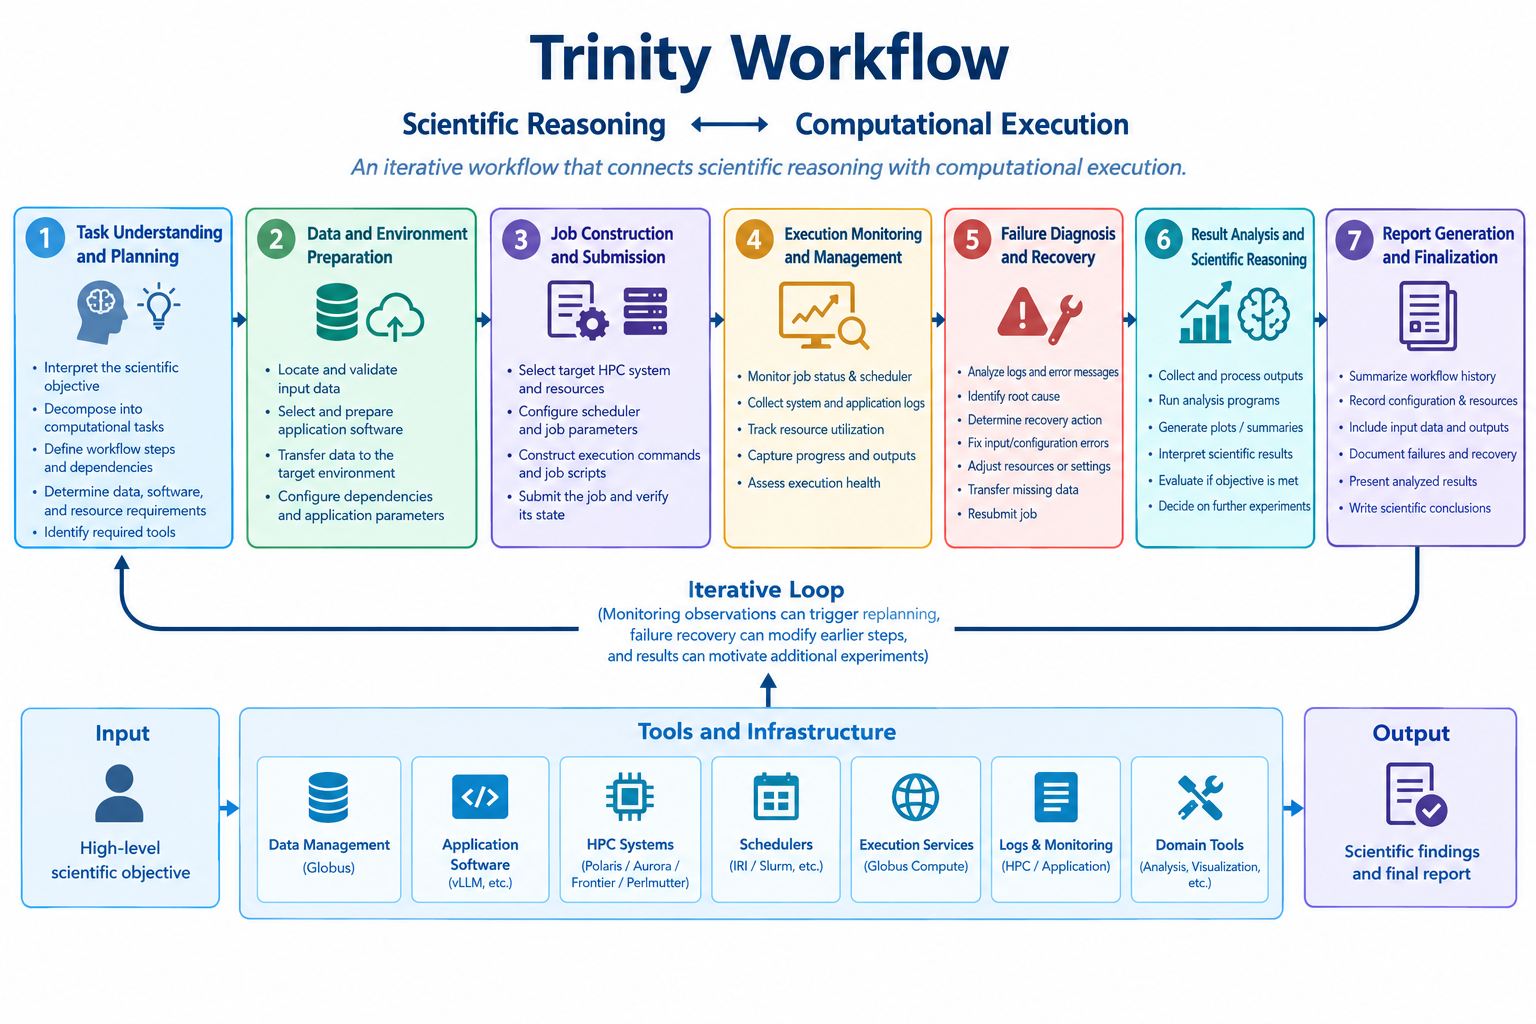
\includegraphics[width=\textwidth,height=0.42\textheight]
        {figures/Trinity_Workflow.png}
    \caption{Overview of the Trinity workflow.}
    \label{fig:Trinity_Workflow}
\end{figure*}

\subsection{Domain-Aware Judging}

The capabilities provided by Trinity are organized into an
iterative workflow that connects \textbf{scientific reasoning with
computational execution}. Given a high-level scientific objective,
the agent determines the computational steps needed to address it,
prepares the required data and software, executes computations on
HPC resources, and reasons over the resulting observations.
Execution is not isolated from reasoning: information collected
during execution can change the agent's understanding of the
workflow state and influence subsequent actions. A workflow may
therefore involve repeated cycles of planning, execution,
monitoring, diagnosis, and scientific reasoning before reaching
a final result.

At a high level, a Trinity workflow consists of
\textbf{task understanding and planning, data and environment
preparation, job construction and submission, execution
monitoring, failure diagnosis and recovery, result analysis and
scientific reasoning, and report generation}. The following
describes each stage and the interactions between them.

\paragraph{Task Understanding and Planning.}
The agent first interprets the user's request to identify the
underlying scientific intent and desired outcome. It decomposes
the objective into computational tasks and establishes a workflow
plan, including the sequence of steps and their dependencies.
The agent also determines the data, software, computational
capabilities, and tools required to carry out the workflow.
At this stage, it identifies requirements rather than committing
to specific input files, software configurations, or HPC resource
allocations. These concrete choices are resolved in subsequent
stages.

\paragraph{Data and Environment Preparation.}
Based on the plan, the agent locates and validates the required
input data, prepares the application software and dependencies,
and configures the execution environment. It may transfer data
to the target computing environment and organize files for
subsequent execution. For workflows involving distributed
resources, the agent can use data-management services such as
Globus to move data between facilities. This stage turns the
workflow's data and software requirements into a usable
computational environment.

\paragraph{Job Construction and Submission.}
With the data and software prepared, the agent determines where
and how to execute the computation. It selects a suitable HPC
system and configures resource requirements, such as the number
of nodes, CPUs, GPUs, memory, and wall time, according to the
application and workflow requirements. The agent then constructs
the job specification, including scheduler parameters, execution
commands, and environment settings. It submits the job through
an HPC execution interface such as IRI or Globus Compute and
verifies that the submission succeeded and that the resulting
execution state is consistent with the planned workflow.

\paragraph{Job Monitoring and Execution Management.}
After submission, the agent observes the execution state and
gathers information needed for subsequent decisions. Monitoring
can include scheduler and job status, HPC system logs, resource
utilization, application logs, execution progress, and generated
outputs. These observations provide both system-level and
scientific context, allowing the agent to determine whether the
computation is progressing normally, has completed, or requires
intervention.

\paragraph{Failure Diagnosis and Recovery.}
Failures are handled as part of the workflow rather than treated
as terminal errors. When an execution step fails or deviates
from expectations, the agent analyzes available evidence,
including scheduler messages, HPC and application logs, error
messages, input data, resource configurations, and previous
workflow actions. It identifies a potential cause and determines
an appropriate recovery action. Depending on the failure,
recovery may involve correcting input or configuration errors,
modifying resource parameters, transferring missing data,
changing execution settings, or resubmitting the job. The
workflow then returns to the relevant preparation, submission,
or monitoring stage.

\paragraph{Result Analysis and Scientific Reasoning.}
Following successful execution, the agent collects and analyzes
the computational results in the context of the original
scientific objective. This stage may involve processing outputs,
running additional analysis programs, generating plots or
summaries, and interpreting application results. The agent
evaluates whether the results sufficiently address the objective
and determines whether additional experiments or computational
steps are necessary. If further work is required, the agent
updates the workflow plan and initiates another execution cycle;
otherwise, it proceeds to report generation.

\paragraph{Report Generation and Finalization.}
Once the agent determines that the scientific objective has been
sufficiently addressed, it consolidates the workflow history and
scientific findings into a final report. The report can include
the original objective, experimental configuration, software and
computational resources, input data, workflow steps, execution
outcomes, failures and recovery actions, analyzed results, and
scientific conclusions. This provides a human-readable record of
both the computational process performed by the agent and the
knowledge obtained from the workflow.

Overall, Trinity combines scientific reasoning with workflow
planning, data and software preparation, HPC resource selection,
tool use, distributed data management, execution monitoring,
failure recovery, and result analysis. The workflow is inherently
iterative: monitoring observations can trigger replanning,
failures can require changes to earlier workflow steps, and
scientific results can motivate additional experiments. This
enables Trinity to move beyond isolated tool invocation toward
end-to-end autonomous execution of complex scientific workflows.



\section{Benchmark Design}\label{sec}

\subsection{Benchmark Overview and Motivation}

Scientific workflows executed by AI agents consist of multiple interdependent subtasks, and failure at any one subtask can prevent successful completion of the entire workflow. For example, an incorrect software selection can lead to invalid input files or an incompatible batch script, while an invalid resource configuration can prevent a correctly prepared application from executing. Evaluating each subtask is therefore important for understanding the reliability of the overall workflow. Moreover, different subtasks may have different capability requirements, making it possible to use lower-cost models for stages that they can complete reliably and reserve more capable models for challenging stages.

We develop an HPC agent benchmark to provide a systematic and reproducible evaluation of these capabilities. The benchmark is designed around the broader Trinity workflow, while the current instantiation focuses on four pre-submission subtasks: software selection, input preparation, resource selection, and batch-job creation. These tasks capture the decisions required to transform a high-level scientific objective into an executable HPC job and provide a controlled starting point for evaluating more complex workflow stages.

A central challenge is that HPC tasks might not have one correct answer. Multiple applications, resource configurations, or workflow artifacts may satisfy the same scientific objective while remaining valid under the constraints of a target system. Therefore, evaluation based on exact answer matching is insufficient. Instead, the benchmark evaluates whether an agent's output satisfies the coupled scientific and system constraints required for successful execution. This requires judging skills that understand both the target scientific application and the characteristics of the HPC environment.

\subsection{Benchmark Tasks and Instances}

We define each benchmark instance as a tuple $(\text{subtask}, \text{application}, \text{HPC system})$. Each subtask contains ten instances spanning diverse HPC systems with different architectures, resource configurations, and batch scheduling environments. The benchmark covers representative scientific applications, including molecular dynamics, quantum chemistry, computational fluid dynamics (CFD), LLM inference, and benchmark applications.

The current benchmark evaluates four pre-submission subtasks:

\begin{itemize}
    \item \textbf{Software selection:} identify an appropriate installed application for the described scientific workload.
    
    \item \textbf{Input preparation:} construct the application-specific input artifacts required for a runnable job without inventing unavailable binaries, runtime files, or unsupported inputs.
    
    \item \textbf{Resource selection:} choose the queue, node count, process configuration, and walltime consistent with system constraints and application scaling guidance.
    
    \item \textbf{Batch-job creation:} construct a scheduler script that requests valid resources and invokes the selected application with the prepared inputs.
\end{itemize}

These subtasks are evaluated individually but remain coupled through their dependencies. For example, the selected application determines the required input format and launch command, while the selected resources must be compatible with both the application and the generated batch script.

The complete Trinity workflow extends beyond job construction. After a batch job is created, the agent can submit it through HPC execution infrastructure and monitor scheduler state, system information, application output, and runtime observations. If execution fails, the agent can diagnose the failure, modify the relevant artifact or configuration, and decide whether to resubmit or take another action. If execution succeeds, the agent can retrieve and analyze the results, determine whether the scientific objective has been achieved, and potentially initiate additional computational steps. The workflow concludes with synthesis and reporting of the configuration, execution history, results, and scientific conclusions. The current benchmark isolates the pre-submission stages to provide a controlled evaluation environment, while future extensions will evaluate monitoring, failure diagnosis and recovery, result analysis, scientific reasoning, report generation, and multi-step workflow execution.

\subsection{Domain-Aware Judging}

\begin{figure*}[t]
    \centering
    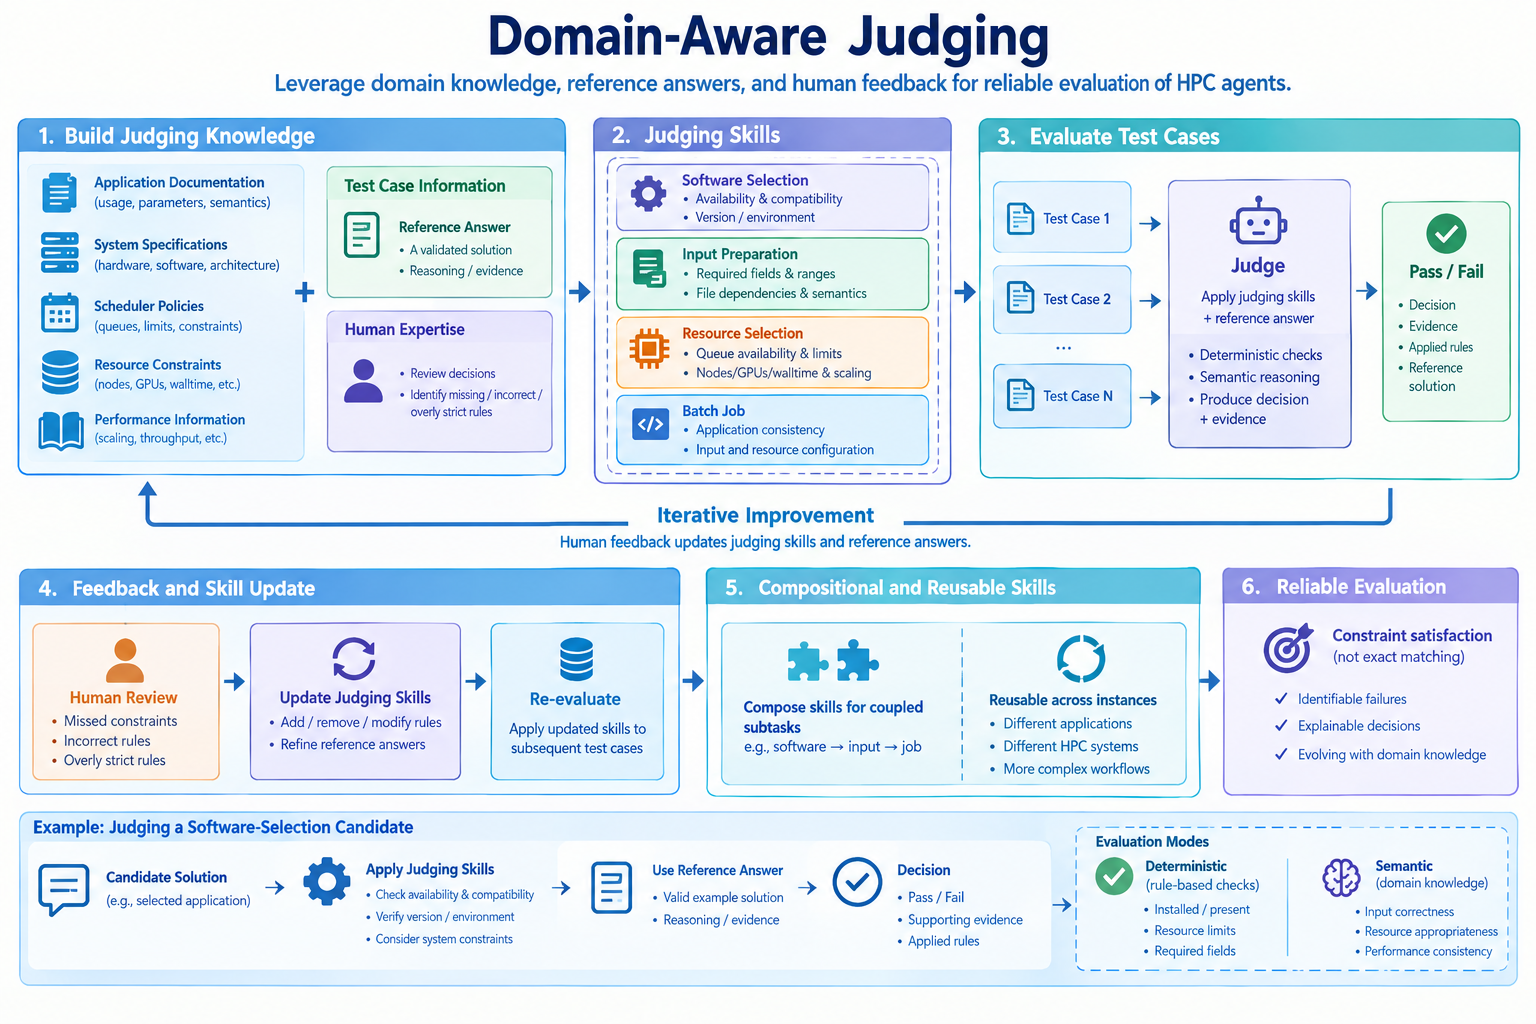
\includegraphics[width=\textwidth,height=0.42\textheight]
        {figures/judging.png}
    \caption{Overview of domain-aware judging.}
    \label{fig:domain-aware-judging}
\end{figure*}

A central challenge in evaluating HPC agents is that correctness cannot generally be determined through exact answer matching. Multiple applications, resource configurations, and workflow artifacts may satisfy the same scientific objective. Determining whether a candidate is valid instead requires knowledge of the target application, input semantics, HPC architecture, scheduler policies, resource limits, and application performance characteristics. A generic language-model judge may recognize a response as plausible without being able to determine whether it can actually execute on the target system.

We therefore develop domain-aware judging skills that capture the rules and evaluation procedures required for each benchmark subtask. The initial judging knowledge is derived from application documentation, system specifications, scheduler policies, resource constraints, input requirements, and application performance information. Each benchmark test case also includes a reference answer that provides a validated example of a correct solution and the reasoning or evidence supporting it. The reference answer provides concrete guidance for what constitutes a valid solution, while the judging rules determine whether alternative solutions that differ from the reference can also satisfy the required constraints.

The judge evaluates a set of benchmark test cases using these judging skills and reference answers, and human experts review the resulting decisions. The review can identify cases where the judge misses a relevant constraint, applies an incorrect rule, or imposes an overly strict rule that incorrectly rejects a valid solution. Based on this feedback, the judging skills are updated by adding, removing, or modifying rules and, when necessary, refining the corresponding reference answers. The updated skills are then evaluated on subsequent test cases. This iterative process allows the judging skills to progressively capture the domain knowledge and flexibility required for reliable evaluation.

Each judging skill specifies what properties should be checked, what evidence should be considered, and which constraints must hold for a candidate to be valid. For example, a software-selection skill verifies application availability and compatibility with the scientific workload. An input-preparation skill checks required fields, valid parameter ranges, file dependencies, and application-specific input semantics. A resource-selection skill evaluates queue availability, node and process limits, walltime constraints, and resource requirements implied by application scaling. A batch-job skill verifies that the script consistently uses the selected application, prepared inputs, and valid resource configuration.

The judging process combines deterministic validation with semantic reasoning. Deterministic checks are applied when a rule can be evaluated directly, such as whether an application is installed, whether requested resources satisfy scheduler constraints, or whether required fields are present in a batch script. Semantic judgment is used when evaluation requires application or scientific knowledge, such as determining whether an input configuration is appropriate for the intended workload or whether a resource configuration is consistent with the application's execution characteristics. The judge records the evidence, rules, and reference solution supporting each decision, allowing human reviewers to identify both missing and overly restrictive rules and update the corresponding judging skills.

The learned judging skills can be reused across benchmark instances and composed when evaluating coupled subtasks. For example, the application selected by the software-selection skill must be compatible with the inputs evaluated by the input-preparation skill and with the launch configuration evaluated by the batch-job skill. The reference answer provides a concrete validated solution for comparison, while the judging rules allow equivalent alternatives to be accepted. This enables correctness to be evaluated as constraint satisfaction rather than textual similarity while making the source of a failure identifiable.

The same learning framework can be extended to later workflow stages. Human feedback can be used to identify missing, incorrect, or overly restrictive rules for job monitoring, failure diagnosis and recovery, result validation, scientific analysis, and report generation. As the benchmark expands, the judging skills and reference answers can therefore evolve with the domain knowledge required to evaluate increasingly complex scientific workflows.

\subsection{Open-Weight Models and Inference-Time Capability Augmentation}

\begin{figure*}[t]
    \centering
    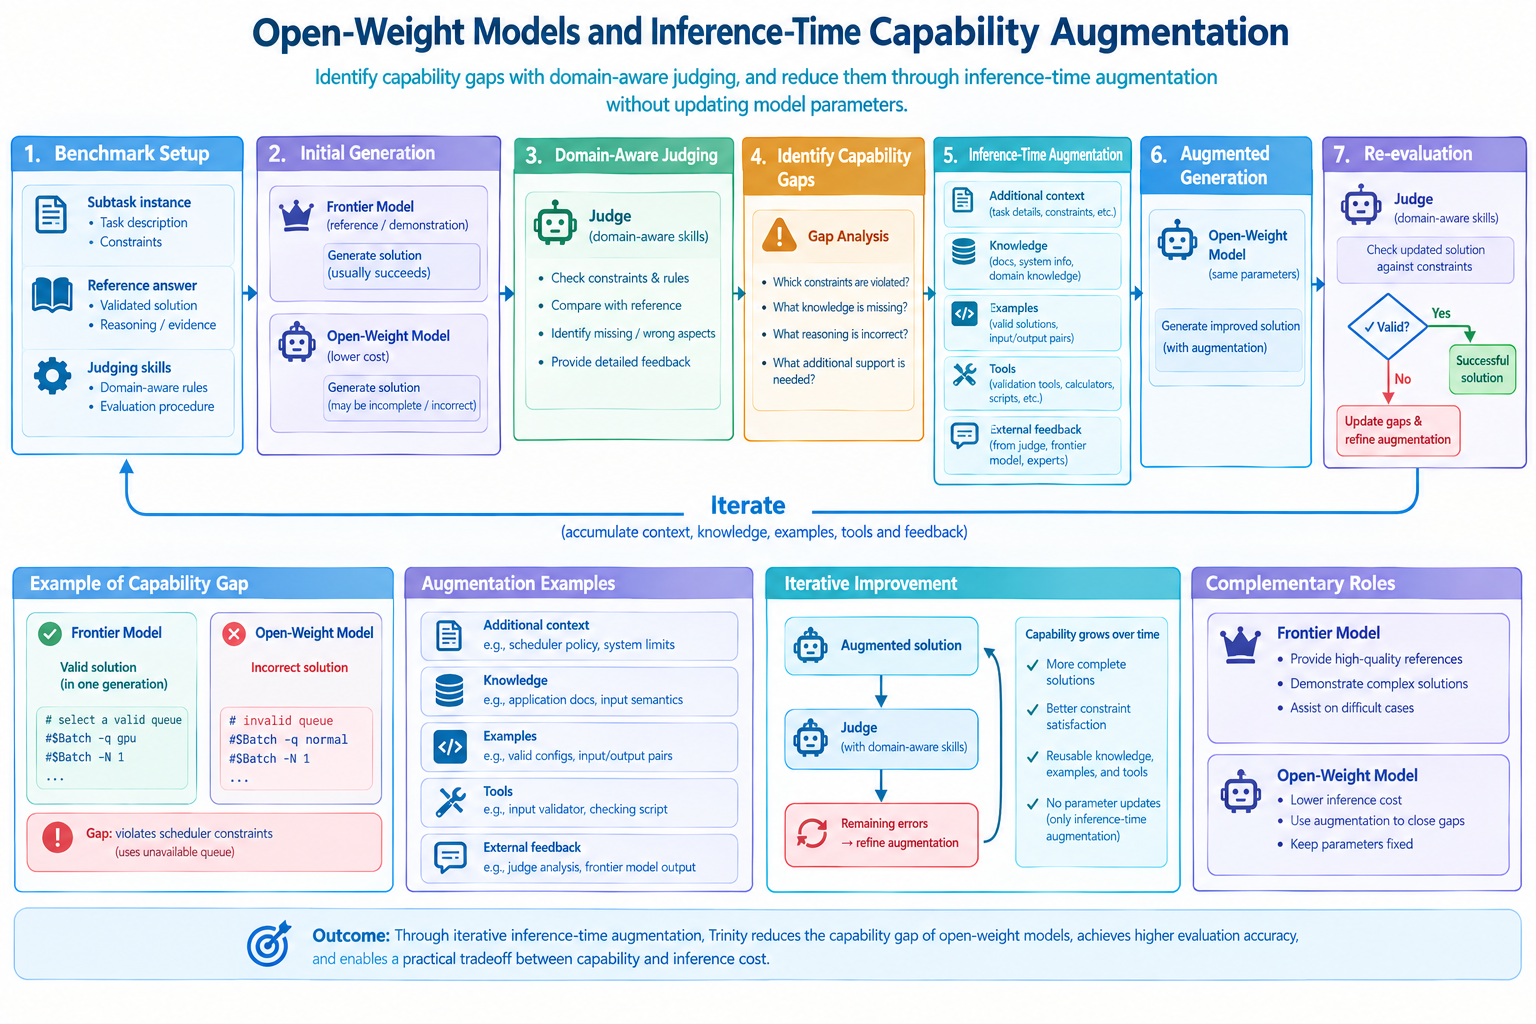
\includegraphics[width=\textwidth,height=0.42\textheight]
        {figures/augmentation.png}
    \caption{Inference-time capability augmentation
    for open-weight models.}
    \label{fig:augmentation}
\end{figure*}

Open-weight models provide a lower-cost alternative to frontier models, but may have weaker capabilities for complex scientific and HPC tasks. For some benchmark instances, a frontier model can produce a valid solution in a single generation, satisfying the relevant scientific and system constraints without additional feedback or external information. In contrast, an open-weight model may produce an incomplete or incorrect solution on the same instance, even when the task is solvable from the information provided in the prompt. This creates a capability gap that does not necessarily require changing the model parameters. Rather than fine-tuning the open-weight model, we investigate whether this gap can be identified and reduced through inference-time capability augmentation, such as providing additional context, examples, tools, or external feedback.

The benchmark provides a mechanism for identifying this gap. For each subtask, a frontier model can first generate a candidate solution, while the domain-aware judging skills evaluate the open-weight model's solution against the same constraints and reference answer. The judge identifies not only whether the solution is incorrect, but also the specific constraints, knowledge, or reasoning requirements that were not satisfied. These observations provide feedback about the capability gap of the open-weight model for the corresponding subtask.

We then use the identified gaps to construct inference-time augmentation for the open-weight model. The augmentation can provide \textit{additional context}, \textit{knowledge}, \textit{examples}, \textit{tools}, or \textit{external feedback}. For example, if an open-weight model selects an invalid HPC queue, the system can provide the relevant scheduler constraints and validated resource-selection examples. If it generates an incorrect application input, retrieved application documentation and valid input examples can be supplied. If the model produces a syntactically valid but semantically incorrect batch script, additional procedural instructions or a validation tool can be introduced. The model parameters remain unchanged throughout this process.

This process is iterative. The augmented open-weight model generates a new solution, and the judging skills evaluate the result again. Remaining errors provide additional evidence about the capability gap and can be used to refine the augmentation. Over successive iterations, the system can accumulate task-specific context, knowledge, examples, tools, and feedback that improve the model's ability to satisfy the required constraints. The resulting capability is therefore obtained through inference-time augmentation rather than parameter updates.

Reference answers and frontier-model outputs play complementary roles in this process. Reference answers provide validated examples of solutions that satisfy the benchmark constraints, while frontier-model outputs can provide additional high-quality demonstrations or candidate solutions for difficult cases. Domain-aware judging skills determine which aspects of these solutions are relevant and identify where the open-weight model differs from a valid solution. This prevents augmentation from simply copying a single reference answer and instead focuses it on the underlying requirements of the task.

This framework enables Trinity to study a practical tradeoff between model capability and inference cost. A lower-cost open-weight model can be used when its augmented capabilities are sufficient for a given subtask, while more capable models can provide references, feedback, or assistance when the open-weight model encounters capability gaps. The benchmark can therefore measure not only the initial capability of different models, but also how effectively their capability gaps can be reduced through reusable inference-time augmentation while keeping their underlying parameters fixed.

\section{Experimental Evaluation}
\label{sec:eval}
 
\subsection{Experimental Setup}
We evaluate four models on the proposed HPC agent benchmark: Nemotron-3-Ultra, Gemma-4-31B, GPT-OSS-120B, and Llama-3.1-8B. The models represent a range of model sizes and capabilities and allow us to examine whether lower-cost open-weight models can reliably perform individual stages of an HPC workflow.
 
The evaluation uses ten benchmark instances for each of the four pre-submission subtasks, resulting in 40 instances. Each instance is evaluated with two prompt configurations, producing 20 attempts per model for each subtask and 320 model responses in total. The two prompt configurations are used to evaluate whether additional context and examples improve model performance. All generated responses are evaluated using the domain-aware judging skills described in Section~\ref{sec:judging}.
 
Each response is evaluated against the requirements of its corresponding benchmark instance. A response passes a subtask only when it satisfies all required judging rules. Individual rule violations are recorded together with their severity, evidence, and the reference solution used by the judge. This provides both an aggregate success measure and a fine-grained view of the failure modes of each model.
 
\subsection{Judging Requirements by Subtask}\label{sec:rubric-detail}
Table~\ref{tab:rubric} summarizes the judging requirements used for each subtask, including their number, severity, and decision method. Each requirement has one of three severity levels. A \emph{fatal} violation assigns a score of 0 regardless of the other requirements; a \emph{major} violation caps the item at 1 out of 2; and a \emph{minor} violation does not prevent the maximum score of 2. Requirements also differ in how they are evaluated. \emph{Deterministic} requirements are checked programmatically against recorded facts, such as an installed-software table, queue node and walltime limits, or the scheduler dialect. \emph{Judge-decided} requirements require semantic assessment of the response, such as determining whether a claim contradicts the catalog or whether a value is consistent with the specified physical system.
\begin{table}[t]
\centering
\caption{Requirements loaded per subtask, by severity and decision method}
\label{tab:rubric}
\begin{tabular}{lccccc}
\toprule
Subtask & Reqs. & Fatal & Major & Minor & Judge \\
\midrule
Software selection & 4 & 1 & 2 & 1 & 2 \\
Input preparation & 25 & 13 & 12 & 0 & 6 \\
Resource selection & 10 & 3 & 6 & 1 & 4 \\
Batch-job creation & 17 & 8 & 8 & 1 & 1 \\
\midrule
Total & 56 & 25 & 28 & 3 & 13 \\
\bottomrule
\end{tabular}
\end{table}
The four subtasks differ substantially in the structure of their requirements. \emph{Input preparation} has the largest rubric, with 25 of the 56 requirements, including 13 fatal requirements. These rules capture concrete properties of application input artifacts, such as required files, mandatory sections, valid keywords, and physical parameter values; 19 of the 25 requirements are therefore evaluated deterministically against the corresponding input-format contract. \emph{Batch-job creation} is similarly dominated by deterministic checks: 16 of its 17 requirements can be evaluated against system and scheduler specifications, including queue availability, walltime limits, node requests, scheduler syntax, and application invocation.
\emph{Resource selection} contains 10 requirements, four of which require judge-based semantic assessment. These include whether resource choices are consistent with the workload and whether supporting claims are appropriately grounded. \emph{Software selection} has the smallest rubric, with four requirements, two of which require semantic judgment. Its requirements focus on selecting the appropriate application and accurately describing its capabilities and availability, rather than requiring exhaustive reproduction of catalog information.
Across all four subtasks, 43 of the 56 requirements (77\%) are evaluated deterministically, while only 13 (23\%) require semantic judgment. Thus, the rubric relies primarily on reproducible checks against recorded application and system facts, while using semantic judgment for cases where exact matching is insufficient. Table~\ref{tab:rule-list} lists all 56 requirements and their severity by subtask. The complete definition of each rule---including its claim, decision method, and rationale---is released as a versioned artifact alongside the benchmark.
\begin{table}[t]
\centering
\scriptsize
\caption{All 56 judging requirements by subtask (superscript: F = fatal, M = major, m = minor)}
\label{tab:rule-list}
\begin{tabular}{@{}p{0.13\linewidth}p{0.83\linewidth}@{}}
\toprule
Subtask & Requirements \\
\midrule
Software (4) & \url{names_one_application}$^{M}$, \url{no_vague_performance_claims}$^{m}$, \url{correct_application}$^{F}$, \url{claims_true_to_catalog}$^{M}$ \\
Input prep. (25) & \url{all_required_files_present}$^{F}$, \url{mandatory_sections_present}$^{M}$, \url{file_identifiable}$^{M}$, \url{exact_filenames_used}$^{M}$, \url{no_output_as_input}$^{M}$, \url{no_binary_contents}$^{F}$, \url{no_truncation}$^{M}$, \url{no_invented_keywords}$^{F}$, \url{values_match_physical_system}$^{M}$, \url{gromacs.tpr_not_authored}$^{F}$, \url{gromacs.grompp_step_stated}$^{M}$, \url{gromacs.mdp_keys_real}$^{F}$, \url{gromacs.required_mdp_fields}$^{M}$, \url{hpl.positional_format}$^{F}$, \url{hpl.header_and_output_lines}$^{F}$, \url{hpl.count_lines_match}$^{F}$, \url{hpl.grid_matches_ranks}$^{M}$, \url{qe.namelist_syntax}$^{F}$, \url{qe.required_namelists}$^{F}$, \url{qe.required_cards}$^{F}$, \url{qe.nat_matches_positions}$^{F}$, \url{qe.ntyp_matches_species}$^{F}$, \url{qe.no_card_terminator}$^{M}$, \url{qe.ibrav_consistent}$^{M}$, \url{qe.pseudopotentials_plausible}$^{M}$ \\
Resource sel. (10) & \url{queue_exists}$^{F}$, \url{no_reservation_queue}$^{M}$, \url{nodes_within_queue_limits}$^{F}$, \url{walltime_within_queue_limit}$^{F}$, \url{ranks_match_build_defaults}$^{M}$, \url{rank_layout_plausible}$^{M}$, \url{rank_arithmetic_consistent}$^{M}$, \url{no_fabricated_evidence}$^{M}$, \url{allocation_matches_scaling_notes}$^{m}$, \url{sizing_not_absurd}$^{M}$ \\
Batch job (17) & \url{filesystems_declared}$^{F}$, \url{walltime_declared}$^{F}$, \url{queue_declared}$^{F}$, \url{select_declared}$^{M}$, \url{account_declared}$^{M}$, \url{queue_exists}$^{F}$, \url{correct_dialect}$^{F}$, \url{no_directive_comments}$^{M}$, \url{invokes_application}$^{F}$, \url{no_placeholders}$^{F}$, \url{inputs_reachable}$^{M}$, \url{slurm.walltime_declared}$^{F}$, \url{slurm.account_declared}$^{M}$, \url{slurm.queue_or_qos_declared}$^{M}$, \url{slurm.nodes_declared}$^{M}$, \url{slurm.no_directive_comments}$^{m}$, \url{slurm.srun_launcher}$^{M}$ \\
\bottomrule
\end{tabular}
\end{table}

\subsection{Results with Unaugmented Prompts}
Without catalog information, performance is low across all four models. Nemotron-3-Ultra and Gemma-4-31B each score $9/40$, while GPT-OSS-120B and Llama-3.1-8B score $5/40$ and $4/40$, respectively. Batch-job creation is nearly unsolved, with only $1/40$ successful cases across all models, while input preparation achieves only $4/40$. The failures fall into two categories: requirements that are consistently violated across models and failures that are more specific to individual models.
\textbf{Failures shared across models.}
Three requirements account for a large fraction of the failures across all four models. The site-specific filesystem directive, \texttt{\#PBS -l filesystems=}, is missing from 31 of 40 batch-job instances and is a fatal requirement. The \texttt{nodes\_within\_queue\_limits} requirement fails on 27 of 40 instances, while \texttt{ranks\_match\_build\_defaults} also fails on 27 of 40. These requirements depend on system-specific information, such as queue node limits, facility-specific scheduler conventions, and the default rank configuration of a local software build.
\textbf{Nemotron-3-Ultra} ($9/40$).
\emph{Software selection} scores $4/10$, with \texttt{claims\_true\_to\_catalog} failing on 5 of 10 instances. For example, for \texttt{nwchem@polaris}, the model claims ``efficient GPU offload for the Fock build,'' even though GPU acceleration is not supported for the cataloged NWChem. \emph{Input preparation} scores $2/10$, with \texttt{values\_match\_physical\_system} failing on 6 of 10 instances and truncated files on 4 of 10. Examples include manifests that enumerate only a few entries followed by an ellipsis despite a stated 100,000-image dataset. \emph{Resource selection} scores $2/10$, with \texttt{ranks\_match\_build\_defaults} failing on 7 of 10 instances; the model frequently selects six ranks per node when the local build default is eight. \emph{Batch-job creation} scores $1/10$, with the required filesystem directive missing from 7 of 10 instances.
\textbf{Gemma-4-31B} ($9/40$).
\emph{Software selection} scores $5/10$. Its main failure is \texttt{correct\_application}, which fails on 4 of 10 instances. For example, on nekRS@Polaris, the model identifies the correct application but also proposes Nek5000 as an alternative, despite the workload's stated A100 requirement. \emph{Input preparation} scores $2/10$: \texttt{values\_match\_physical\_system}, \texttt{mandatory\_sections\_present}, and \texttt{no\_invented\_keywords} each fail on 4--6 of 10 instances. For example, the model produces an input file with physical parameters that do not match the stated system and introduces configuration keywords that are not part of the application's input format. \emph{Resource selection} scores $2/10$, with \texttt{queue\_exists} failing on 6 of 10 instances and \texttt{nodes\_within\_queue\_limits} on 7 of 10. One recurring example is the use of a nonexistent \texttt{theta} queue on Polaris. \emph{Batch-job creation} scores $0/10$; the filesystem directive is missing in 8 of 10 instances, and the charge account is missing in 3 of 10.
\textbf{GPT-OSS-120B} ($5/40$).
\emph{Software selection} scores $4/10$, with \texttt{claims\_true\_to\_catalog} failing on 5 of 10 instances. \emph{Input preparation} scores $0/10$. The most common failure is \texttt{no\_invented\_keywords}, which fails on 6 of 10 instances. It also produces abbreviated files on 3 of 10 instances. \emph{Resource selection} scores $1/10$, with \texttt{no\_fabricated\_evidence} failing on 6 of 10 instances. For example, the model states that ``measured runs on similar Cray-GPU systems typically finish in 2--5 minutes'' despite having no runtime measurements in the prompt. \emph{Batch-job creation} scores $0/10$. The filesystem directive is missing in 8 of 10 instances, while comments are placed on scheduler-directive lines in 6 of 10 instances.
\textbf{Llama-3.1-8B} ($4/40$).
\emph{Software selection} scores $3/10$, with \texttt{correct\_application} failing on 6 of 10 instances. For example, for \texttt{nwchem@polaris}, the model selects Psi4, a real and plausible quantum-chemistry code, instead of NWChem, the application specified for the system. \emph{Input preparation} scores $0/10$: \texttt{all\_required\_files\_present} and \texttt{mandatory\_sections\_present} each fail on 9 of 10 instances. Rather than producing the required \texttt{.par}, \texttt{.re2}, and \texttt{.udf} artifacts, the model frequently substitutes an invented \texttt{nekrs\_input.in} file. \emph{Resource selection} scores $1/10$, with \texttt{nodes\_within\_queue\_limits} failing on 9 of 10 instances and walltime limits on 8 of 10. \emph{Batch-job creation} scores $0/10$. The model frequently uses the wrong PBS dialect, for example specifying \texttt{\#PBS -l nodes=1=4} instead of the required \texttt{select=} syntax, with this failure occurring on 8 of 10 instances.
Overall, the unaugmented prompts expose different failure modes across the four subtasks. Software selection is affected by unsupported or unverifiable claims about available software; resource selection frequently violates system-specific queue, node, and build constraints; batch-job creation repeatedly omits required scheduler directives; and input preparation often produces incomplete artifacts or artifacts in the wrong format. These failures occur despite the models receiving the same task instances, indicating substantial sensitivity to the system-specific details required by the benchmark.

\subsection{Results with Augmented Prompts}
With the scientific application and system context restored in the prompt, performance improves substantially for all four models, although the magnitude of improvement varies. Nemotron-3-Ultra reaches $31/40$ (+22), Gemma-4-31B reaches $28/40$ (+19), GPT-OSS-120B reaches $22/40$ (+17), and Llama-3.1-8B reaches $18/40$ (+14). Batch-job creation and resource selection show the largest gains, improving from $1/40$ to $29/40$ and from $6/40$ to $31/40$, respectively. In contrast, input preparation improves only from $4/40$ to $10/40$ and remains the weakest subtask for every model.
\textbf{Improvements shared across models.}
The system-specific requirements that dominated the unaugmented failures are largely resolved when the scientific application and system context is supplied. Missing filesystem directives decrease from 31/40 to 0/40 instances, \texttt{queue\_exists} failures from 18/40 to 0/40, \texttt{nodes\_within\_queue\_limits} failures from 27/40 to 3/40, and \texttt{ranks\_match\_build\_defaults} from 27/40 to 4/40. These requirements correspond directly to information explicitly provided in the augmented prompts, including the per-queue node limits, required filesystem list, and build-specific default rank counts. The large reductions therefore show that providing system-specific information substantially improves compliance with these constraints.
\textbf{Nemotron-3-Ultra} ($31/40$, $+22$).
Batch-job creation is solved ($10/10$), and resource selection is nearly solved ($9/10$); software selection improves to $8/10$. However, some failures persist even when the relevant application and system information is explicitly available. For example, \texttt{claims\_true\_to\_catalog} still fails on \texttt{qe@aurora}: the model asserts ``Intel Xe GPU (XPU) accelerators via SYCL/DPC++ offload,'' although the supplied context records \texttt{gpu\_support: false} for that build. \texttt{no\_vague\_performance\_claims} also fails on 3 of 10 instances, including an assertion that PyTorch ``minimizes overhead and complexity'' without supporting evidence. Input preparation remains the main weakness at $4/10$; the model continues to invent configuration keywords not defined by the target format, such as NekRS \texttt{[STATISTICS]} blocks and a lowercase \texttt{targetWalkers} in a QMCPACK DMC block where the keyword is case-sensitive.
\textbf{Gemma-4-31B} ($28/40$, $+19$).
The largest gains are in resource selection and batch-job creation, which reach $9/10$ and $8/10$, respectively, compared with $2/10$ and $0/10$ without the context. Software selection reaches $8/10$; the earlier \texttt{correct\_application} failure on nekRS@Polaris, where the model proposed Nek5000 despite the stated A100 requirement, does not recur in the augmented prompt. Input preparation remains the main weakness at $3/10$. In particular, \texttt{values\_match\_physical\_system} fails on 5 of 10 instances even though the relevant physical parameters are explicitly provided. For example, the model produces a QE cell definition with \texttt{ibrav=2} and \texttt{celldm(1)=10.26} corresponding to a 5.43\,\AA{} primitive cell rather than the requested 8.716\,\AA{} $2\times2\times2$ supercell. Similarly, it produces a GROMACS ion count corresponding to 0.27\,M NaCl when the target concentration is 0.15\,M. These errors arise from incorrect numerical reasoning rather than missing application or system information.
\textbf{GPT-OSS-120B} ($22/40$, $+17$).
Resource selection is solved ($10/10$), and batch-job creation improves to $5/10$, but software selection remains unchanged at $4/10$. The model continues to assert, for \texttt{qe@aurora}, that the installed build provides ``Intel oneAPI SYCL off-loading ... PVC accelerators,'' contradicting the \texttt{gpu\_support: false} field explicitly provided in the context. Thus, supplying the application and system context does not improve this particular software-selection failure. A second persistent defect occurs in batch-job creation: \texttt{no\_directive\_comments} fails on 4 of 10 instances, with the corresponding Slurm-dialect criterion failing on 2 more. The model continues to append explanatory comments to \texttt{\#PBS}/\texttt{\#SBATCH} directive lines despite the scheduler conventions provided in the prompt.
\textbf{Llama-3.1-8B} ($18/40$, $+14$).
Software selection improves from $3/10$ to $9/10$: given an explicit list of installed applications, the model generally selects the correct application, avoiding the plausible-but-wrong substitutions observed in the unaugmented prompt, such as selecting Psi4 for an NWChem task. Batch-job creation improves to $6/10$, although \texttt{invokes\_application} still fails on 3 of 10 instances. For example, the model invokes AlphaFold as \texttt{srun -n 1 -G 1 python /global/.../bin/python run\_alphafold.py}, using one Python executable to execute another Python executable as a script. Resource selection remains weak at $3/10$: \texttt{rank\_arithmetic\_consistent} fails on 3 of 10 instances, with stated ranks and GPU counts that are mathematically inconsistent. For example, the model specifies 128 total ranks and one GPU per rank while the request requires two GPUs. Input preparation remains at $0/10$, unchanged from the unaugmented prompt; the model continues to substitute incorrect file formats for the artifacts required by the application.
Taken together, the augmented results show that supplying scientific application and system context and examples substantially improves compliance with explicit system constraints, particularly for resource selection and batch-job creation. However, several failure modes persist even when the relevant information is present in the prompt. These include incorrect interpretation of application and system information, numerical inconsistencies, invented application-specific syntax, and malformed command construction. The results therefore distinguish failures caused by missing context from failures that persist despite that context being explicitly available.
 
\subsection{Discussion}
The experimental results highlight two important properties of AI agents for HPC workflows. First, capability is strongly dependent on the specific workflow stage. A model may be effective at identifying software or constructing scheduler scripts while failing at application-specific input preparation. Second, many failures are not general language-generation errors but violations of concrete scientific or system constraints. These failures motivate domain-aware judging rather than generic response evaluation.
 
The results also show why evaluating only end-to-end success can obscure useful information. The subtask-level benchmark identifies whether a failure originates from application selection, scientific input construction, resource configuration, or scheduler integration. The judging rules further identify the specific violated constraint. This provides a direct mechanism for diagnosing the capability gap of an individual model.
 
Finally, the initial context-and-example augmentation experiment provides a foundation for evaluating richer inference-time mechanisms. These mechanisms can include reusable procedural skills, retrieval-augmented knowledge, tool-assisted validation, frontier-model feedback, and iterative refinement, while keeping the underlying open-weight model unchanged.

\section{Conclusion}\label{sec}

We presented \textit{Trinity}, a multi-agent framework that connects LLM-based reasoning with scientific applications, HPC systems, execution infrastructure, and scientific feedback. Within Trinity, we developed a benchmark for four foundational pre-submission capabilities: software selection, input preparation, resource selection, and batch-job creation. The benchmark evaluates constraint satisfaction rather than textual similarity, enabling multiple valid solutions and subtask-level analysis through domain-aware judging skills refined with human feedback. Evaluation across 80 instances shows substantial variation across workflow stages, with input preparation presenting a particularly challenging capability gap. These results highlight the need for domain-specific knowledge and capability augmentation beyond general language-model capabilities. Future work will extend the benchmark to execution monitoring, failure diagnosis, result analysis, and scientific reasoning, moving toward evaluation of complete autonomous scientific workflows.


% ============================================================
% Acknowledgments
%
% DO NOT include identifying information in the double-anonymous
% submission. Add acknowledgments only in the appropriate
% camera-ready version.
% ============================================================

% \section*{Acknowledgment}
% [Acknowledgments for camera-ready version.]


% ============================================================
% References
% ============================================================

\bibliographystyle{IEEEtran}
\bibliography{references}

\end{document}
```
